%% AZIENDA OSPITANTE
\chapter{Azienda ospitante}\label{chap:company}

\section{Profilo dell'azienda}
\begin{figure}[H] 
	\centering
	
\includegraphics[scale=0.3]{zextras}
	\caption{Logo Zextras s.r.l.}
	\label{fig:logoZextras}
\end{figure}
L'attività di stage descritta in questo elaborato è stata svolta presso l'azienda Zextras s.r.l. nella sede a Torri Di Quartesolo (VI). \\
Questa società è nata nel 2011 con l'obbiettivo di espandere le possibilità della suite di prodotti di collaborazione Zimbra (sez. \ref{subsec:Zimbra}), uno dei sistemi collaborativi (posta elettronica, calendario, contatti …) più diffusi al mondo. Ha dato così vita a Zextras Suite (sez. \ref{subsec:Zextras}), un insieme di estensioni per Zimbra Collaboration che migliorano i servizi già presenti e offrono funzionalità importanti per un uso lavorativo del software.
In pochi anni è riuscita a rendere la propria suite di prodotti l'estensione professionale per Zimbra Open Source più avanzata tra le soluzioni di collaborazione sul mercato. I loro prodotti sono riconosciuti come ottimali anche dall'azienda proprietaria Synacor, la quale ha portato ad una collaborazione per lo sviluppo di alcuni prodotti open source e per Zimbra Suite Plus.
Ad oggi l'azienda presenta sedi secondarie in paesi, quali Francia, Brasile, Russia e Stati Uniti;  inoltre, possiede partner in tutto il mondo.\\


\subsection{Zimbra} \label{subsec:Zimbra}
\begin{figure}[H] 
	\centering
	
\includegraphics[scale=0.2]{zimbra}
	\caption{Logo Zimbra}
	\label{fig:logoZimbra}
\end{figure}
Zimbra è un server di workgroup open source che mette a disposizione una suite di software collaborativi che consentono di condividere documenti e attività. 
Di base essa offre i seguenti servizi:
\begin{itemize}
	\item configurazione personalizzata,
	\item gestione della posta elettronica,
	\item rubriche, calendari e condivisione di file,
	\item chat e chiamate vocali,
	\item integrazione con i canali web
	\item privacy e alti livelli di sicurezza
	\item disponibilità per i dispositivi mobili: oltre che mediante client Zimbra Web e attraverso i client di posta elettronica tradizionale, è possibile accedere alle e-mail, ai calendari e alle altre offerte da dispositivi mobile. 
\end{itemize}
Le funzionalità di Zimbra possono essere facilmente estese grazie alla possibilità di creare ed aggiungere degli add-on chiamati Zimlet. Esse sono delle integrazioni che permettono di personalizzare i servizi ed integrarli con servizi web e applicazioni di terzi.
Zimbra è disponibile in due versioni: 
\begin{itemize}
	\item Zimbra Open Source Edition: soluzione completamente open source ma con disponibili solo le funzionalità standard;
	\item Zimbra Network Edition: soluzione completa di tutte le funzionalità sia per l'amministratore di sistema sia per l'utente finale.
\end{itemize}


\subsection{Zextras Suite} \label{subsec:Zextras}
Zextras Suite è un Add-On per Zimbra Collaboration: i suoi prodotti sono progettati per espandere le funzioni di Zimbra Open Source Edition in maniera a se stante rispetto i moduli Zimbra Network Edition. Infatti Zextras Suite non è distribuito assieme ad alcun binario o sorgente sotto il copyright di Zimbra. \\
Le principali innovazioni che sono state portate nel mondo Zimbra riguardano la sicurezza dei dati, la mobilità e la gestione dello storage.\\
La suite comprende i seguenti prodotti:
	\begin{itemize}
		\item Zextras Backup: modulo di backup professionale che permette il salvataggio dei dati in realtime;
		\item Zextras Mobile: modulo per la gestione e sincronizzazione di email, contatti, eventi e task con qualsiasi device mobile tramite Exchange ActiveSync;
		\item Zextras Powerstore: modulo per la gestione avanzata di storage locali e remoti, così da ottimizzare i volumi dei dati Zimbra e risparmiare spazio attraverso la compressione e la deduplicazione;
		\item Zextras Admin: interfaccia amministrativa avanzata per monitorare gli utenti e le funzionalità di Zimbra, Zextras Suite e ogni altro Zimlet;
		\item Zextras Chat: piattaforma client/server integrata in Zimbra per la messaggistica istantanea e le videochat.
	\end{itemize}

\begin{figure}[H] 
	\centering
	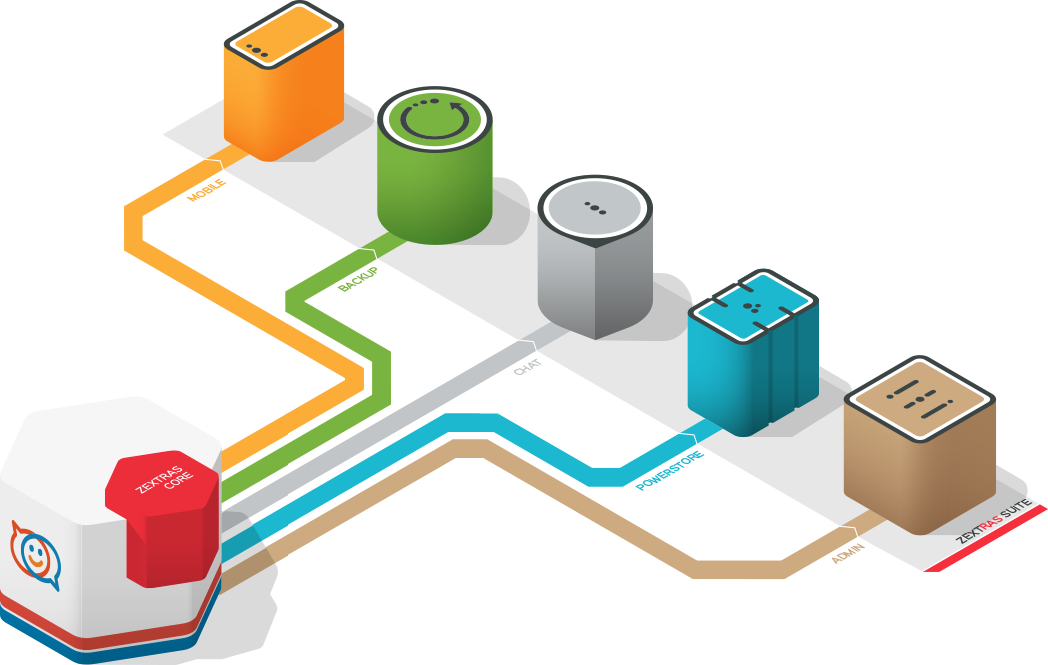
\includegraphics[scale=0.3]{zextras_2018}
	\caption{Rappresentazione Zextras suite}
	\label{fig:modulizextras}
\end{figure}
Come rappresentato in figura~\ref{fig:modulizextras}, Zextras suite è un'estensione modulare per Zimbra Open Source che può essere applicata secondo le proprie esigenze. Proprio per questo risulta la migliore scelta per un uso professionale di Zimbra.

\section{Metodo di lavoro}
La necessità di sviluppare progetti particolarmente complessi che si unisce all'esigenza di mantenere una certa flessibilità e trasparenza, ha portato l'azienda a preferire l'utilizzo di un ciclo di sviluppo del software di tipo \emph{agile}, rispetto a metodi di management più tradizionali incentrati sui processi di sviluppo ma non reattivi ai cambiamenti. Questi, infatti, causerebbero una maggior dispersione di risorse, soprattutto nel caso di una forte interazione con il cliente.\\
La filosofia dello sviluppo agile si basa su quattro pilastri fondamentali che caratterizzano.  Esse sono:
\begin{itemize}
	\item gli individui e le interazioni sono più importanti dei processi e degli strumenti;
	\item è più importante avere del software funzionante rispetto ad avere una documentazione esaustiva;
	\item è più importante la collaborazione col cliente che il rispetto dei contratti;
	\item bisogna essere pronti a rispondere ai cambiamenti oltre che aderire alla pianificazione.
\end{itemize}
Questi principi sono ampiamente condivisi dalla compagine aziendale, la quale basa lo sviluppo dei propri prodotti sulla continua interazione con gli stakeholder e con i clienti.

\subsection{Scrum}
In particolare  viene utilizzato il metodo Scrum, che oltre ad essere uno dei sistemi più diffusi, è particolarmente adatto a progetti complessi ed innovativi.\\
Lo Scrum prevede un modello di sviluppo iterativo nel quale ogni ciclo viene definita uno \emph{Sprint}: esso è un periodo di tempo, solitamente di durata compresa tra 1 a 4 settimane, nel quale viene prefissata una lista di requisiti e funzionalità che devono essere implementate in tale periodo.
Questa lista di funzionalità e requisiti viene definita prima in una \emph{Product Backlog}, documento che contiene tutti i requisiti necessari per la realizzazione del progetto, e poi, periodicamente, in una \emph{Sprint Backlog}, documento nel quale vengono definiti tutti i task da completare nei singoli sprint.
L'azienda prevede sprint di due settimane e la fine di ogniuno di essi coincide con una release del software.
Per gestire al meglio sprint e backlog di ogni progetto vengono eseguite delle riunioni periodiche di diverse tipologie:
\begin{itemize}
	\item \textbf{Sprint Planning}: riunione che precede l'inizio del progetto in cui si stila la Product Backlog e si determina il numero e la durata degli sprint in base al tempo a disposizione e agli obiettivi. Viene inoltre definita la Sprint Backlog per il primo sprint;
	\item \textbf{Daily Scrum}: breve confronto giornaliero che permette di sincronizzare i lavoro di tutto il team e di affrontare tempestivamente i problemi riscontrati;
	\item \textbf{Sprint Review}: revisione al termine di ogni sprint che serve a valutare se gli obiettivi prefissati sono stati completati in modo esaustivo o se è necessario modificare la pianificazione del lavoro per lo sprint successivo;
\end{itemize}

\subsection{Strumenti a supporto di processi e servizi} \note{Si potrebbero mettere le icone/simboli dei vari software}
Zextras S.r.l. utilizza la suite Atlassian, composta da una serie di prodotti atti al miglioramento dello sviluppo del software, della gestione dei progetti e della collaborazione. 
\subsubsection{BitBucket Server}
Per il versionamento del software viene utilizzato BitBucket Server, un servizio di self-hosting per repository Git e per il controllo delle versioni. Permette di eseguire tutte le operazioni di base di Git di base (è un servizio simile a GitHub) ed in più consente un pieno controllo dell'accesso in lettura e scrittura al codice. L'accesso può essere differenziato per utente o per gruppi. BitBucket Server, essendo un servizio di self-hosting, ha la particolarità di poter essere eseguito nei server locali così da preservare la riservatezza del proprio codice. Inoltre permette l'integrazione con altri strumenti sviluppati dall'azienda Atalassian, tra i quali \hyperref[subsubsec:jira]{Jira}, \hyperref[subsubsec:bamboo]{Bamboo} e \hyperref[subsubsec:confluence]{Confluence}.
\subsubsection{Jira}\label{subsubsec:jira}
Jira è un prodotto di issue-tracking che fornisce funzionalità quali tracciamento dei bug, rilevamento dei problemi e gestione di progetti. Questo software permettere di scegliere il tipo di ciclo di sviluppo con cui si preferisce gestire il progetto: nel caso dell'azienda Zextras si adatta perfettamente alla metodologia di lavoro scelta e al sistema Scrum, in quanto permette di gestire al meglio gli sprint e le relative backlog.
\subsubsection{Bamboo}\label{subsubsec:bamboo}
Bamboo è un server sviluppato da Atalassian per la continuous integration e deployment. Tra le varie funzionalità, permette di eseguire più build in parallelo, per un completamento più rapido, e in caso di errori di compilazione fornisce un'analisi dell'errore, inclusa la stack trace.
\subsubsection{Confluence}\label{subsubsec:confluence}
Confluence è un software di collaborazione per la creazione di documenti che permette di creare, organizzare e lavorare su materiale condiviso. È uno strumento che permette di centralizzare le informazioni, tenere traccia di ogni modifica e, inoltre, permette una gestione granulare dei permessi di accesso ad ogni singolo file.

